\documentclass[acmsmall,review,anonymous]{acmart}\settopmatter{printfolios=true,printccs=false,printacmref=false}
\acmJournal{PACMPL}
\acmVolume{1}
\acmNumber{OOPSLA} % CONF = POPL or ICFP or OOPSLA
\acmArticle{1}
\acmYear{2018}
\acmMonth{1}
\acmDOI{} % \acmDOI{10.1145/nnnnnnn.nnnnnnn}
\startPage{1}
\setcopyright{none}
\bibliographystyle{ACM-Reference-Format}
\citestyle{acmauthoryear}   %% For author/year citations
\usepackage{my_style}
\usepackage{listings, wrapfig,xspace}
\usepackage{paralist}
\usepackage{booktabs} % To thicken table lines

\lstset{language=R}
\definecolor{LightGray}{rgb}{.92,.92,.92}
\definecolor{Gray}{rgb}{.3,.3,.3}
\definecolor{DarkGray}{rgb}{.5,.5,.5}
\lstset{ %
  columns=flexible,
  captionpos=b,
  frame=single,
  framerule=0pt,
  tabsize=2,
  belowskip=0.5em,
  backgroundcolor=\color{LightGray},
  basicstyle=\small\ttfamily,
  emphstyle=,
  keywordstyle=,
  commentstyle=\color{Gray}\em,
  stringstyle=\color{Gray},
%  numbers=left,
  showstringspaces=false
}
\lstdefinestyle{R}{ %
  language=R,
  morekeywords={assign, delayedAssign},
  deletekeywords={env, equal, c, runif, trace, args, exp, t, all},
  breaklines=true
}
\lstdefinestyle{Rin}{ %
  style=R,
  breaklines=false
}
\renewcommand{\k}[1]{{\tt #1}\xspace}


\newcommand{\eg}{\emph{e.g.},\xspace}
\newcommand{\ie}{\emph{i.e.},\xspace}
\newcommand{\cf}{\emph{cf.}\xspace}

\newcommand{\PIR}{\textsf{PIR}\xspace}
\newcommand\pirI[1]{\mathtt{#1}}
\renewcommand{\c}[1]{{\lstinline[style=Rin]!#1!}\xspace}
\newcommand{\code}[1]{{\lstinline[style=Rin]!#1!}\xspace}
% Macros for type names from the old paper.
\newcommand{\attr}[2]{\ensuremath{#1_{\mathtt{#2}}}\xspace}
\newcommand{\attrclass}[3]{\ensuremath{#1^{\mathtt{#3}}_{\mathtt{#2}}}\xspace}
\renewcommand{\to}{\ensuremath{\rightarrow}\xspace}


\renewcommand{\null}{\texttt{\textbf{null}}\xspace}
\newcommand{\scalar}{\texttt{\textbf{scalar}}\xspace}
\renewcommand{\vector}{\texttt{\textbf{vector}}\xspace}
\newcommand{\class}{\texttt{\textbf{class}}\xspace}
\newcommand{\any}{\texttt{\textbf{any}}\xspace}
\newcommand{\environment}{\texttt{\textbf{env}}\xspace}
\newcommand{\expression}{\texttt{\textbf{expression}}\xspace}
\newcommand{\Language}{\texttt{\textbf{lang}}\xspace} %% Upper case!
\newcommand{\externalptr}{\texttt{\textbf{externalptr}}\xspace}
\renewcommand{\symbol}{\texttt{\textbf{symbol}}\xspace}
\newcommand{\pairlist}{\texttt{\textbf{pairlist}}\xspace}
\newcommand{\weakref}{\texttt{\textbf{weakref}}\xspace}
\renewcommand{\int}{\texttt{\textbf{int}}\xspace}
\newcommand{\chr}{\texttt{\textbf{chr}}\xspace}
\newcommand{\dbl}{\texttt{\textbf{dbl}}\xspace}
\newcommand{\lgl}{\texttt{\textbf{lgl}}\xspace}
\newcommand{\clx}{\texttt{\textbf{clx}}\xspace}
\newcommand{\raw}{\texttt{\textbf{raw}}\xspace}
\newcommand{\NA}{\texttt{{NA}}\xspace}
\newcommand{\VARGS}{\texttt{\textbf{...}}\xspace}
\newcommand{\T}{\ensuremath{T}\xspace}
\renewcommand{\S}{\ensuremath{S}\xspace}
\newcommand{\V}{\ensuremath{V}\xspace}
\newcommand{\A}{\ensuremath{A}\xspace}
\newcommand{\ID}{\ensuremath{ID}\xspace}
\newcommand{\F}{\ensuremath{F}\xspace}
\newcommand{\B}{\ensuremath{B}\xspace}
\newcommand{\FUN}[2]{\ensuremath{\langle #1 \rangle \rightarrow #2}\xspace}
\newcommand{\STRUCT}[1]{\texttt{\textbf{struct}}\ensuremath{\langle #1\rangle}\xspace}
\newcommand{\LIST}[1]{\texttt{\textbf{list}}\ensuremath{\langle #1\rangle}\xspace}
\newcommand{\CLASS}[1]{\texttt{\textbf{class}}\ensuremath{\langle #1\rangle}\xspace}
\newcommand{\VEC}[1]{#1\k{[]}\xspace}
\newcommand{\NAVEC}[1]{\k{\string^}\!#1\k{[]}\xspace}

\newcommand{\contractr}{{\sf ContractR}\xspace} % contractr
\newcommand{\roxygen}{{\sf Roxygen2}\xspace} % roxygen
\newcommand{\typetracer}{{\sf Typetracer}\xspace} % typetracer
\newcommand{\rdt}{{\sf R-dyntrace}\xspace}
\newcommand{\covr}{{\sf Covr}\xspace}



\newcommand {\PercUnitypedPositions} {87.2\%\xspace} %% 0.8717
\newcommand {\PercManytypedPositions} {2\%\xspace} %% 0.018
\newcommand {\CountMonomorphicFunctions} {13.1 K\xspace} %% 13099
\newcommand {\PercMonomorphicFunctions} {64.8\%\xspace} %% 0.648016226377758
\newcommand {\CountPolymorphicFunctions} {7.1 K\xspace} %% 7115
\newcommand {\PercPolymorphicFunctions} {35.2\%\xspace} %% 0.351983773622242

\newcommand{\CranAssertsRnd}{32.3K\xspace}
\newcommand{\CranAsserts}{32,327\xspace}
\newcommand{\CranAssertsInPackagesRnd}{2.4K\xspace}
\newcommand{\CranAssertsInPackages}{2,363\xspace}
\newcommand{\CranAssertsInFunctionsRnd}{15.9K\xspace}
\newcommand{\CranAssertsInFunctions}{15,929\xspace}
\newcommand{\CranStopifnotRatio}{87.6\%\xspace}
\newcommand{\CranTypedAssertsRnd}{12K\xspace}
\newcommand{\CranTypedAsserts}{11,997\xspace}
\newcommand{\CranTypedAssertsRatio}{37.1\%\xspace}
\newcommand{\CranTypedAssertsPackagesRnd}{1.5K\xspace}
\newcommand{\CranTypedAssertsPackages}{1,487\xspace}
\newcommand{\CranTypedAssertsPackagesRatio}{62.9\%\xspace}
\newcommand{\CranTypedAssertsFunctionsRnd}{7.1K\xspace}
\newcommand{\CranTypedAssertsFunctions}{7,119\xspace}
\newcommand{\CranTypedAssertsFunctionsRation}{44.7\%\xspace}
\newcommand{\CranPartiallyTypedAssertsRnd}{15.5K\xspace}
\newcommand{\CranPartiallyTypedAsserts}{15,487\xspace}
\newcommand{\CranPartiallyTypedAssertsRatio}{47.9\%\xspace}
\newcommand{\CranPartiallyTypedAssertsPackagesRnd}{1.7K\xspace}
\newcommand{\CranPartiallyTypedAssertsPackages}{1,664\xspace}
\newcommand{\CranPartiallyTypedAssertsPackagesRatio}{70.4\%\xspace}
\newcommand{\CranPartiallyTypedAssertsFunctionsRnd}{9K\xspace}
\newcommand{\CranPartiallyTypedAssertsFunctions}{9,045\xspace}
\newcommand{\CranPartiallyTypedAssertsFunctionsRation}{56.8\%\xspace}
\newcommand{\CorpusAssertsRnd}{2K\xspace}
\newcommand{\CorpusAsserts}{1,995\xspace}
\newcommand{\CorpusAssertsInPackages}{153\xspace}
\newcommand{\CorpusAssertsInFunctionsRnd}{1.3K\xspace}
\newcommand{\CorpusAssertsInFunctions}{1,264\xspace}
\newcommand{\CorpusStopifnotRatio}{94.7\%\xspace}
\newcommand{\CorpusTypedAssertsRnd}{1K\xspace}
\newcommand{\CorpusTypedAsserts}{1,005\xspace}
\newcommand{\CorpusTypedAssertsRatio}{50.4\%\xspace}
\newcommand{\CorpusTypedAssertsPackages}{114\xspace}
\newcommand{\CorpusTypedAssertsPackagesRatio}{74.5\%\xspace}
\newcommand{\CorpusTypedAssertsFunctions}{688\xspace}
\newcommand{\CorpusTypedAssertsFunctionsRation}{54.4\%\xspace}
\newcommand{\CorpusPartiallyTypedAssertsRnd}{1.2K\xspace}
\newcommand{\CorpusPartiallyTypedAsserts}{1,223\xspace}
\newcommand{\CorpusPartiallyTypedAssertsRatio}{61.3\%\xspace}
\newcommand{\CorpusPartiallyTypedAssertsPackages}{125\xspace}
\newcommand{\CorpusPartiallyTypedAssertsPackagesRatio}{81.7\%\xspace}
\newcommand{\CorpusPartiallyTypedAssertsFunctions}{859\xspace}
\newcommand{\CorpusPartiallyTypedAssertsFunctionsRation}{68\%\xspace}
\newcommand{\AssertthatRevdeps}{211\xspace}
\newcommand{\AssertrRevdeps}{2\xspace}


\begin{document}
\title{Designing Types for R, Empirically}

\newcommand{\NUMFUNCTIONS}{20,214\xspace}  %%% TODO auto-gen
\newcommand{\NUMPACKAGES}{412\xspace}  %%% TODO auto-gen
\newcommand{\PACKAGES}{412\xspace}  %%% TODO auto-gen
\newcommand{\genthat}{genthat\xspace}  %%% TODO auto-gen
\newcommand{\YEARS}{20\xspace} %%TODO fix
\newcommand{\PERCFAILEDASSERTIONS}{2.19\%\xspace}
\newcommand{\PERCFAILEDASSERTIONSWUNDEF}{2.23\%\xspace}
\newcommand{\PERCASSERTIONSUNDEF}{0.04\%\xspace}
\newcommand{\NUMPKGSEVAL}{7485\xspace} % autogenerate
\newcommand{\NUMASSERTIONS}{62,171,573\xspace} %autogenerate
\newcommand{\PROPFUNSFAILEDCHECK}{21.21\%\xspace}
\newcommand{\PROPFUNSFAILEDCHECKNOSTHREE}{15.48\%\xspace} 
\newcommand{\PROPARGSFAILINGASSERTS}{3.53\%\xspace} % autogen....
\newcommand{\PERCSUCCARG}{96.46\%\xspace}
\newcommand{\PERCSUCCFUNNOSTHREE}{84.52\%\xspace}
\newcommand{\PERCSUCCFUNS}{78.79\%\xspace}
\newcommand{\PERCCALLSBADFUNSINTESTS}{5.38\%\xspace}
\newcommand{\TOTNUMSIGS}{21,730\xspace}
\newcommand{\PROPSTRUCTSDYN}{44.46\%\xspace}
\newcommand{\NUMFILESRUN}{145,373\xspace}


\begin{abstract}
The R programming language is widely used in a variety of domains.  It was
designed to favor an interactive style of programming with minimal syntactic
and conceptual overhead. This design is well suited to interactive data
analysis, but a bad fit for tools such as compilers or program analyzers
which must generate native code or catch programming errors.  In particular,
R has no type annotations, all operations are dynamically checked at
run-time. The starting point for our work are the twin questions, \emph{what
  expressive power is needed to accurately type R code?} and \emph{which
  type system is the R community willing to adopt?} Both questions are
difficult to answer without actually experimenting with a type system. The
goal of this paper is to provide data that can feed into that design
process. To this end, we perform a large corpus analysis to gain insights in
the degree of polymorphism exhibited by idiomatic R code and explore
potential benefits that the R community could accrue from a simple type
system.  As a starting point, we infer type signatures for \NUMFUNCTIONS
functions from \NUMPACKAGES packages among the most widely used open source
R libraries.
\end{abstract} \maketitle

\section{Introduction}

Our community builds, improves, and reasons about programming languages.  To
make design decisions that benefit users, we need to understand our target
language as well as the real-world needs it answers. Often, we can appeal to
our intuition, as many languages are intended for general purpose
programming tasks. Unfortunately, intuition may fail when looking at
domain-specific languages as these languages designed for a specific group
of users to solve very specific needs. This is the case of the data science
language R.

R and its ancestor S were designed, implemented, and maintained by
statisticians. Originally they aimed to be glue languages for reading data
and calling statistical routines written in Fortran. Over three decades they
became widely used across many fields for data analysis and visualization.
Modern R, as an object of study, is fascinating. It is a vectorized,
dynamically typed, lazy functional language with limited side-effects,
extensive reflective facilities and retrofitted object-oriented programming
support.

Many of the design decisions that gave us R were intended to foster an
interactive, exploratory, programming style. These include, to name a few,
the lack of type annotations, the ability to use syntactic shortcut, and the
automatic conversion between data types.  While these choices have led to a
language with a low barrier to entry---many data science educational
programs do not teach R itself but simply introduce some of its key
libraries---they have also created a language where errors can go
undetected.

Retrofitting a type system to the R programming language would increase our
assurance in the result of data analysis. But, we are faced with two
challenges. First, it is unclear what would be the \emph{right} type system
for a language as baroque as R. For example, one of the most popular data
type, the \code{data.frame}, is manipulated through reflective operations --
a data frame is a table whose columns can be added or removed on the fly.
Second, but just as crucially, designing a type system that will be adopted
would require overcoming some prejudices and educating large numbers of
users.

This paper is a data-driven study of what a type system for the R language
could look like. Our intention is to eventually propose changes to the
language, but we are aware that for any changes to be accepted by the user
community they must clearly benefit the language without endangering
backwards compatibility. Our goal is thus to find a compromise between
simplicity and usefulness; any proposed type system should cover common
programming idioms while remaining easy to learn and to use.

This paper focuses on a simpler problem than an entire type system, instead,
we limit the scope of our investigation to giving types to function
signatures. In order to do this, we design a simple type language, one that
matches the R data types but omits features such as parametric polymorphism
and subtyping between user-defined data types. We then extract type
signature from execution traces of a corpus of widely used libraries.  This
allows us to see how far one can get with the simple type language and
identify limitations of our this particular design. We validate the
robustness of the extracted type signature by implementing a contact system
that weaves the types around their respective functions, and use a large
number of clients of the target packages for validation. The contract system
can be used by the R community to experiment with our type signatures and to
replace ad hoc error checking code.

To sum up, our paper makes the following main contributions:
\begin{itemize}
\item We implemented tooling to automatically extract type signatures from R
  functions and to instrument R functions with checks based on their declared
  types. The tooling is robust and scalable to the entire R language.
\item We carried out a large-scale analysis of corpus of \PACKAGES widely
  used and actively maintained libraries to extract function type signatures and
  validated the robustness of the inferred type signatures against \NUMFILESRUN
  programs that use those functions.
\item We report on the appropriateness and usefulness of a simple type
  language for the R programming language.
\end{itemize}

Our tools are open source and publicly available on GitHub (link anonymize),
all results in this paper are reproducible and will be submitted for
artifact evaluation should this paper be accepted.
%
\section{Background} %%%%%%%%%%%%%%%%%%%%%%%%%%%%%%%%%%%%%%%%%%%%%%%%%%%%%%%%%

In this section, we introduce related work on extending dynamic languages
with static type system and we give a short primer on the R programming
language.

\subsection{Related Work}

Dynamic programming languages such as Racket, JavaScript and PHP have been
extended post-facto with various static type systems.  In each case, the
type system was carefully engineered to match the salient characteristics of
the host languages and to foster a particular programming style. For
example, Typed Racket emphasizes functional programming and support the
migration from untyped to fully typed code~\cite{tf-popl08},
Hack~\cite{hack13} and TypeScript~\cite{BAT14} focus on typing
object-oriented features of PHP and JavaScript, respectively. They allow to
intersperse typed and untyped code in a fine-grained manner.

But what if the design of the type system is unclear?  \citet{tip} propose
an intriguing approach called trace typing. With trace typing, a new type
system can be prototyped and evaluated by applying the type rule to
execution traces of programs. While the approach has the limitation of
dynamic analysis techniques, namely that the results are only as good at the
coverage of the source code, it allows to quickly test new design and
quantify how much of a code base can be type-checked.  Other approaches that
infer types for dynamic analysis include the work of \citet{FurrAF2009} for
Ruby.

There is no previous work on types for the R programming language. We take
inspiration in the above mentioned works but focus on adapting them to our
target language.


\subsection{The R Programming Language} %%%%%%%%%%%%%%%%%%%%%%%%%%%%%%%%%

The R Project is a key tool for data analysis.  At the heart of the R
project is a \emph{vectorized, dynamic, lazy, functional, object-oriented}
programming language with a rather unusual combination of
features~\cite{ecoop12} designed to ease learning by non-programmer and
enable rapid development of new statistical methods.  The language was
designed~\citet{R96} as a successor to S~\cite{S88}.

In this paper, we will attempt infer type signature for functions. We now
introduce some relevant concepts.  Functions can be called with named
parameters, arguments can have default values, and R also support variable
argument lists.  To illustrate all of this in a single example, consider:

\begin{lstlisting}
  f <- function(x, ..., y=if(z==0) 1, z=0) x + y + if (missing(...)) 0 else c(...)
\end{lstlisting}

\noindent
This function four formal parameters, \k x, \k{...}, \k y and \k z. Argument
\k x can be bound positionally or passed by name. The vararg argument,
\k{...}, is always passed positionally. The remaining two arguments must be
passed by name.  Arguments \k y and \k z have default values, in the case of
\k z this is a constant, but \k{y}'s default value is an expression that
depends on the value of \k z. The body of the function will add parameters
\k x and \k y with either the scalar 0 or the result of concatenating the
varargs into a primitive vector. The function \k{missing} tests if an
argument was explicitly passed. The following are some valid invocations
of \k f:

\begin{lstlisting}
 > f(1)    
 [1] 2             % a double vector, y is 0, ... is missing
 > f(1,2) 
 [1] 4             % a double vector, y is 0, ... is 2
 > f(1,2,3)
 [1] 4 5           % a double vector, y is 0, ... is 2, 3
 > f(2,3,x=1)
 [1] 4 5           % a double vector, y is 0, ... is 2, 3
 > f(x=1, y= 1)
 [1] 2             % a double vector, y is 1, ... is missing
 > f(x=1, z= 1)
 numeric(0)        % a double vector of length 0, y is NULL
 > f(1L,2L,y=1L)
 [1] 4             % an integer vector, y is integer 1, ... is integer 2
 > f(1, y=c(1,2))
 [1] 1 2           % a double vetor, y is 1, 2, ... is missing
\end{lstlisting}

\noindent
The above hints at the polymorphism of the language, \k f, may return a
vector of integer or of double, the length of the vector depends on the
length of the varargs and of \k x and \k y.  The language does not really
differentiate between scalar and vectors.  Some more exotic types that can
be encountered include vectors of complex number and list of arbitrary
types. Function \k f can be invoked with those as well.

\begin{lstlisting}
 > c1 <- complex(re=1, im=2)
 > c2 <- complex(re=2, im=1)
 > f(c1)
 [1] 1             % a double vector, x is complex, y is double
 > f(c1,y=c2)
 [1] 2+1i          % a complex vector, x and y are complex
 > l1 <- list(1,2)
 > l2 <- list(c1,c2)
 > f(l1) 
 [1] 1             % a double vector, x is a list of doubles
 > f(l1,y=l2)
 [[1]]             % a list of complex, x is a list of doubles
 [1] 1+2i          %                      y is a list of complex
 
 [[2]]
 [1] 2+1i
\end{lstlisting}

R has one builtin notion of type that can be queried by the \k{typeof}
function. Figure~\ref{rtypes} lists all of the builtin types that are
provided by the language. They are the possible return values of
\k{typeof}. There is no intrinsic notion of subtyping in R. But, in many
context a \k{logical} will convert to \k{integer}, and an \k{integer} will
convert to \k{double}.  Some odd conversions can occur in corner cases, such
as \k{1<"2"} holds and \k{c(1,2)[1.6]} returns the first element of the
vector, as the double is converted to an integer. R does not distinguish
between scalars and vectors (they are all vectors), so \code{typeof(5) ==}
\code{typeof(c(5)) == typeof(c(5,5))} \code{ == "double"}. Finally all
vectorized data types have a distinguished missing value denoted by
\code{NA}. The default type of \code{NA} is \k{logical}. We can see that
\code{typeof(NA)=="logical"}, but NA inhabits every type:
\code{typeof(c(1,NA)[2])=="double"}.

\begin{wrapfigure}{r}{6.1cm}
\footnotesize\begin{tabular}{l@{}l@{}}\hline
\bf Vectors:\\\hline
\k{logical}   & vector of boolean values\\
\k{integer}   & vector of 32 bit integer values\\
\k{double}    & vector of 64 bit floating points\\
\k{complex}   & vector of complex values\\
\k{character} & vector of strings values\\
\k{raw}       & vector of bytes\\
\k{list}      & vector of values of any type\\\hline
{\bf Scalars:}\\\hline
\k{NULL}      &  singleton null value\\
\k{S4}        &  instance of a S4 class \\
\k{closure}   &  function with its environment\\
\k{environment}& mapping from symbol to value \\\hline
{\bf Implementation:}\\\hline
\k{special},
\k{builtin}, &\k{symbol}, \k{pairlist}, \k{promise}\\
\k{language}, \k{char}, \k{...}, & \k{~any}, \k{expression},\\
\k{externalprt},& \k{bytecode}, \k{weakref}\\\hline
\end{tabular}\caption{Builtin Types}\label{rtypes}\end{wrapfigure}

With one exception all vectorized data types are monomorphic, the exception
is the \k{list} type which can hold values of any other type including
\k{list}. For all monomorphic data types, attempting to store a value of a
different type will cause a conversion. Either the value is converted to the
type of vector, or the vector is converted to the type of the value.

Over the years, programmers have found the need for a richer type structure
and have added {\it attributes}. The best way to think of attributes is as
an optional map from name to values that can be attached to any object.
Attributes are used to encode various type structures. They can be queried
with functions such as \k{attributes} and \k{class}.  The addition of
attributes lets programmers extend the set of types by tagging data with
user-defined attributes. For example, one could define a vector of four
values, \code{x<-c(1,2,3,4)} and then attach the attribute \k{dim} with a
pair of numbers as value: \code{attr(x,"dim")<-c(2,2)}.  From that point,
arithmetic functions will treat \k{x} as a 2x2 matrix. Another attribute
that can be set is the \k{class}.  This attribute can be bound to a list of
class names. For instance, \code{class(x)<-"human"}, set the class of \k{x}
to be \k{human}.  Attributes are thus used for object-oriented
programming. The S3 object system support single dispatch on the class of
the first argument of a function, whereas the S4 object system allows
multiple dispatch (on all arguments). Some of the most widely used data
type, such as data frames, leverage attributes. A data frame, for instance,
is a list of vectors with a class and a column name attribute.

Scalar data types include the distinguished \k{NULL} value, which is also of
type \k{NULL}, instance of classes written using the S4 object system,
closures and environments.  The implementation of R has a number of other
types listed in Figure~\ref{rtypes} for reference.

%%%%%%%%%%%%%%%%%%%%%%%%%%%%%%%%%%%%%%%%%%%%%%%%%%%%%%%%%%%%%%%%%%%%%%%%%%%%%%
\section{Designing A Type Language for R}%%%%%%%%%%%%%%%%%%%%%%%%%%%%%%%%%%%%%

This section sets out to propose a candidate design for a type language to
describe the arguments and return values of functions in R.  The goal is not
to get a final design but rather a starting point for an iterative process.
Fig.~\ref{types} presents our type language. An early design choice was to
stay close to the R language and only depart in small, hopefully,
non-controversial ways.  Functions types have the form \FUN{A_1, \dots,
  A_n}\T where each $\A_i$ argument is either a type \T or \VARGS, a
variable length argument list. The rest of this section details and
motivates our design.

\begin{figure}[!h] \noindent \small  \centering\begin{minipage}{.45\linewidth}
\begin{tabular}{lclr}
\T& ::= & \any          & \it top type\\
  & |   & \null         & \it null type\\
  & |   & \environment  & \it environment type \\
  & |   & \S            & \it scalar type \\
  & |   & \V            & \it vector type \\
  & |   & \T~\k{|}\T    & \it union type \\
  & |   & \k{?} \T      & \it nullable type \\
  & |   & \FUN{A_1, ..., A_n}\T    & \it function type \\
  & |   & \LIST\T                  & \it list type\\
  & |   & \CLASS{ID_1, ..., ID_n}  & \it class type\vspace{5pt}\\
\end{tabular}\end{minipage}   \hfill
\begin{minipage}{.45\linewidth}\begin{tabular}{lclr}
\A & ::= & \T          & \it arguments \\
   & |   & \VARGS      & \vspace{5pt} \\
\V & ::= & ~\VEC\S     & \\
   & |   & \NAVEC\S    & \it na vector types \vspace{5pt}\\
\S & ::= & \int        & \\
   & |   & \chr \\
   & |   & \dbl \\
   & |   & \lgl \\
   & |   & \clx \\
   & |   & \raw \vspace{5pt}\\
\end{tabular}\end{minipage}\caption{The R type language}\label{types}
\end{figure}

\paragraph{Scalar vs. Vectors} We distinguish between
vectors of length 1, and vectors of any dimension. The base types, \int,
\dbl, \clx, \lgl (booleans), \chr, and \raw (bytes), can be either vectors
(e.g., \VEC\int) or scalars (e.g., \int).  A vector can happen to be of
length 1, and thus a scalar value is also a vector.  Vectors are
homogeneous, in that a vector of doubles contains only doubles.

\paragraph{NA values} In R, a value can be \emph{not available}, written
\NA. Each of basic types has its specific \NA. Thus there is an \int \NA as
well as a double \NA, and they are different.  The type system allows to
distinguish between vectors that may contain {\NA}s(written \NAVEC\int) and
those who are guarantee to be \NA-free (\VEC\int).  A \NA-free vector can be
treated as a vector that may {\NA}s.  We do not allow scalar values to be
\NA and the type \raw does not allow {\NA}s.

\paragraph{Unions} We support untagged unions of types written
$\T_1 \k{~|~} \T_n$.

\paragraph{Nullables} 
The \null type is inhabited by a singleton \code{NULL} value often used as a
sentinel or a stand in for arguments with no value.  To capture this
behavior, we introduce a nullable type \code{?}\T.  The difference between
the \NA and \code{NULL} values is that the latter cannot be stored in
vectors.

\paragraph{Lists} Heterogeneous collections are implemented using lists.
Lists and vectors are closely related: a vector converts to a list with
\code{as.list}, and lists to vectors with \code{unlist} (coercions may
ensue). The list type is parameterize, \LIST\T, when the list is
heterogeneous \T defaults to \any.

\paragraph{Classes} 
R has more than one notion of type. Values can be attributed, one important
attribute is the class of a value.  A class is a list of names that are used
to mimic object-oriented programming. The type system includes class types
written \CLASS{\ID_1,\dots,\ID_n}.

\paragraph{Environments}
Environments are lists with reference semantics: mutating a value in an
environment is performed in-place.  They are used to store variables and to
escape from the copy-on-write semantics of other data types. 


\section{Extracting and Checking Signatures}

For this paper, we have built tooling to (\emph{a}) automate the extraction
of raw type signatures from execution traces, (\emph{b}) infer type
signatures from a set of raw types, and (\emph{c}) validate the inferred
signatures by the means of contracts. This section presents each step
of this pipeline.

\subsection{Extracting raw type signature from traces}

We implemented \typetracer, an automated tool for extracting raw type
signatures from execution traces of R programs. The goal of this tool is to
output a tuple $\langle f, t_1, \dots, t_n, t\rangle$ for each function call
during the execution of a program, where $f$ is an identifier for a
function, $t_i$ are type-level summaries of the arguments and $t$ is a
summary of the return value.

While this task is seemingly simple, the details and their proverbial devil
are surprisingly tricky to get right and to scale to long running programs.
To avoid starting from scratch, our implementation reuses an open source
dynamic analysis framework for R named \rdt~\cite{oopsla19} which consists
of an instrumented R Virtual Machine based on GNU-R version 3.5.0. The
framework exposes hooks at key points in the R interpreter to which user
defined callbacks can be attached. These hooks include function entry and
exit, method dispatch for the S3 and S4 object systems, the longjumps used
by the interpreter to implement non-local exit, creation and forcing of
promises (lazy evaluation), variable definition, value creation, mutation
and garbage collection.

\paragraph{Raw types}
The type information output by the tool includes the \emph{type tag} of each
value. The R internal types are translated to names in the proposed type
system. The next bit of information output is the \emph{class} which is an
optional list of names, it may be absent, and, in some cases, it may be
implicit (i.e. the interpreter blesses some values with the \k{matrix} and
\k{array} classes even when they have no attributes). 
Depending on the value's type tag, the tool collects further information:

\begin{itemize}
\item For vectors, the number of dimensions and the present of \NA values.
\item For lists, a recursive traversal collects element types.
\item For promises, we attempt to establish the type of its result or output
  \any.
\end{itemize}

\noindent
To obtain raw types, we make use of R's C FFI and use low-level machinery to
collect type tags and attributes from the R run-time.  The types that we
provide to users are constructed during post-processing, and rely on the
detailed information made available by these low-level reflection
mechanisms.

\paragraph{Varargs}
Arguments that are part of a function's varargs (denoted \VARGS) are
ignored, as type \VARGS is output as the type of the entire varargs construct.


\paragraph{Promises}
The fact that arguments are evaluated lazily (in that expression are packed
into promises and evaluated on first access) complicates the information
gathering.  For example, some promises remain un-evaluated, and it would be
erroneous to force them as they may cause side-effects that will affect the
programs execution.  To deal with unevaluated arguments, we make an initial
guess for each argument at function entry.  If the promise is later forced,
we simply update the recorded type for the argument.

\paragraph{Missing arguments}
Parameters which receive no values when the function is called are termed
missing. This occurs when a function was called with too few arguments and
no default value was specified for missing arguments.  We record a
\k{missing} type for such argument.  There are two obvious ways to deal with
missing arguments: type them as \any or type them as some unit type.  As we
are performing a dynamic analysis, we conservatively type them as
\LIST{\any}.

\paragraph{Non-local returns}
When a function exits with a longjump there is no return value to speak
of. In order to ensure that call traces are valid when a longjump occurs, we
intercept the unwinding process initiated by the longjump and mimic the
functionality of the functions being exited. When no return value is present
for a call, we record a special \k{jumped} return type.

\paragraph{Implementation details.}
We primarily rely on eight callbacks: \k{closure\_entry}, \k{closure\_exit},
\k{builtin\_entry}, \k{builtin\_exit}, \k{special\_entry},
\k{special\_exit}, \k{promise\_force\_entry}, and
\k{prom\-ise\_force\_exit}.  The function-related callbacks are used mainly
for bookkeeping: the analysis is notified that a construct has been entered
by pushing the call onto a stack.  The calls themselves store a trace
object, it is that object that holds the type information. As R can perform
single or multiple dispatch on function arguments depending on their class,
the relevant information is kept by the {\tt \_entry} variants.



\subsection{Inferring type signatures from raw types}

The output of the \typetracer tool consists of a set of tuples of raw types,
each representing a function call in some program's execution. The inference
step consolidates the different tuples corresponding to a particular function
definition across multiple programs and distills them into a single type
signature.  The shape of the inferred function signatures is:

\medskip
\FUN{ T_{1,1} \k{~|~} T_{1,i}, \dots, T_{n,1} \k{~|~} T_{n,j}}{T_1\k{~|~} T_k}
\medskip

\noindent
In other words, we take the union of the types occurring at individual
argument positions rather than an union of function types. Furthermore, we
apply some transformation on the types to keep the size of types in check.

\medskip
\begin{tabular}{rclll}
  \T \k{~|~} \T  & $\Rightarrow$ &  \T &  \\
  \T \k{~|~} $T'$ & $\Rightarrow$ &  \T & \it{iff} $T' <: T$  \\
  \LIST{\T} \k{~|~} $\LIST{T'}$ & $\Rightarrow$ &  \LIST\T & \it{iff} $T' <: T$  \\
   $\null \k{~|~} \VEC{\S_1} \k{~|~}\dots \VEC{\S_n}$  & $\Rightarrow$ &
  $ \NAVEC{\S_1} \k{~|~}\dots \NAVEC{\S_n}$ &  \\
  \\
  \\
  \NAVEC\S  & <:& \VEC\S \\
  \T        & <:& \k{?}\T \\
  \LIST{\T} & <:& \LIST{\T'} & \it{iff} \T <: \T' \\
  \S        & <:& \VEC\S \\
  \lgl      & <:& \int\\
  \int      & <:& \dbl\\
  \dbl      & <:& \clx\\  
\end{tabular}
\medskip

\noindent
Assuming that type sequences can be reordered freely, we rewrite types to
minimize their size by removing redundant types, types that are subsumed by
subtyping, and \null types. For performance reasons, we bound lists to no
more than five types in their union, above that they become \LIST{any}.
Functions are alos limited to twenty arguments. Higher-order functions are
approximated by \any to \any.

\subsection{Checking types signatures with contracts}

One way to validate the inferred type annotations is to check that different
programs using one of the functions for which a type signature has been
inferred respect the signature.  \contractr is an R package that allows to
decorate function with assertions. We use it to insert type checks of the
arguments and return values. As usual with R, this is not straightforward.

While \contractr's primary logic has been implemented in C++ to reduce its
runtier overhead, we have not observed a single segfault during our use of
the package.  It has been tested with GNU R-3.5.0 and hardened with a
battery of 400 test cases. It works by modifying function definition to
insert a call to a type-checking function.

In terms of usability, our checker is enabled automatically whenever a
package is loaded in R. So, a simple invocation of \code{library(contractr)}
causes contracts to be injected in all packages.  On loading, \contractr
scans all packages in the user's workspace and inserts contracts in
functions for which type signatures are available. Then \contractr sets up
package load hooks which are executed when new packages are loaded.
Furthermore, \contractr automatically removes contracts from all functions
and restores them to their original state when it is unloaded.
The type signatures can be provided externally, in a file, thus avoiding the
need to change the source code of checked packages.  Type declarations can
also be written alongside a \code{@type} section inside \roxygen function
comment blocks. \roxygen is an R package that enables authors to add
documentation. The documentation sections are processed by \roxygen before
package build and a registered method for each custom tag section is
invoked with the section data and documented object. \contractr uses this
mechanism to register a hook for a custom \code{@type} tag. 
The \contractr API allows users to explicitly insert contracts during
interactive development by supplying the type signature as a string.
Contracts can be removed by calling \code{remove\_contract}.  Contracts can
be selectively enabled or disabled for code blocks by wrapping them in calls
to \code{ignore\_contracts} and \code{capture\_contracts}.  These functions
return a data frame that contains all the information about failed and
successful contract assertions in the wrapped code blocks.  Multiple
failures can introduce noise; this is avoided by setting
\code{contractr.severity} to \code{'silence'}.  \contractr still performs
type-checking so that results can be obtained by calling
\code{get\_contracts}. Setting \code{contractr.severity} flag to
\code{'error'} turns the type-checking warnings to errors and
halt the program.

\paragraph{Checking the values} A number of properties can be checked
by a simple tag check, namely whether a value is a: null, environment, vector
or scalar. Other properties require an inspection of the contents of a
value: the absence of \NA or the type of the elements of list. Union types
require checking for each of the alternatives. We do not check higher-order
functions in this version of the tool.
When argument values are wrapped in promises (this is not always the case
due to compiler optimizations), in order to retain the non-strict semantics
of R, the expression held in the promise is wrapped in a call to the type
checker, and type checking is delayed until the promise is forced. This
leads to corner cases such that the type checking of a function may happen
after that function has returned.
Return values require care as well.  Functions return the last expression
they evaluate, thus to avoid having to analyze the code of the called
function the checker will register a callback on the exit hook. The hook is
executed in the function call's environment. Another wrinkle is due to
longjumps which causes active function calls on the stack to be
discarded. When they are discarded, their exit hooks are called.  But, these
function do not have a return value to type-check. \contractr deals with
this problem by allocating a unique sentinel object which serves as the
return value for calls that are discarded. The exit hook does not call the
type-checker if it see the sentinel.

%%%%%%%%%%%%%%%%%%%%%%%%%%%%%%%%%%%%%%%%%%%%%%%%%%%%%%%%%%%%%%%%%%%%%%%%%%%%%
\section{Project Corpus}\label{sec:corpus} %%%%%%%%%%%%%%%%%%%%%%%%%%%%%%%%%%

For this paper we have selected \CorpusLoadable packages consisting of
\CorpusRCodeRnd lines of R code and \CorpusNativeCodeRnd lines of native
code (C/Fortran). Figure~\ref{fig:corpus} shows these packages, the size of
the dots reflects the project's size in lines of code including both R and
native code\footnote{Lines of source code reported excludes comments and
  blank lines, counted by \emph{cloc}, \cf
  \url{https://github.com/AlDanial/cloc}}, the x-axis indicates the
expression code coverage in percents and the y-axis gives the number of
reverse dependencies in log scale. Dotted lines indicate means. Packages
with over \PackageSizeOutierRnd lines of code are annotated.

\begin{figure}[!h]\centering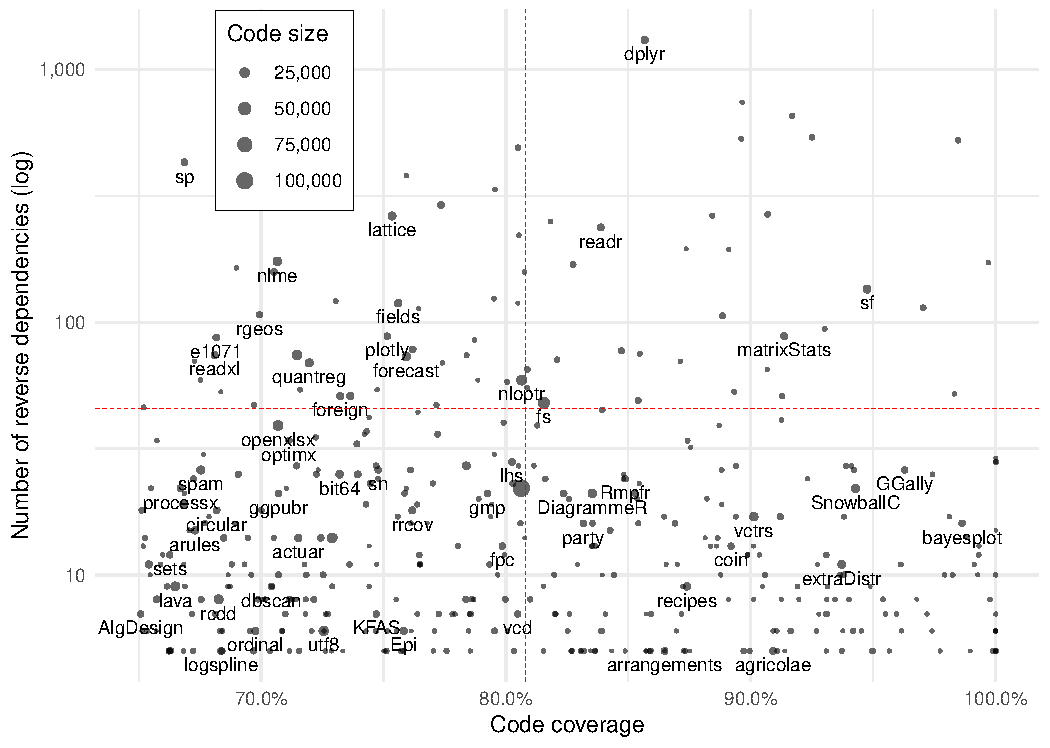
\includegraphics[width=.8\linewidth]
  {plots/corpus.pdf}\caption{Corpus}\label{fig:corpus}
\end{figure}

These packages come from the Comprehensive R Archive Network
(CRAN\footnote{\url{http://cran.r-project.org}}), the largest repository of R
code with over \AllCranRnd packages\footnote{CRAN receives about 6 new package
  submissions a day~\cite{Ligges2017}} containing over \AllRCodeRnd and
\AllNativeCodeRnd R and native code respectively. Unlike other open code
repositories such as GitHub, CRAN is a curated repository. Each submitted
package must abide to a number of well-formedness rules that are automatically
checked asserting certain quality. Most relevant for this work is that all of
the runnable code (including code snippets from examples and vignettes) is
tested and only a successfully running package is admitted in the archive.

We have downloaded and installed all available CRAN packages. Out of the
\AllCranRnd packages, we managed to install \AllLoadableRnd. The main reason for
this is that \rdt is based on R 3.5.0 and some of the packages are no longer
compatible with this version. Some packages also require extra native
dependencies which were not present on our servers. We defined two criteria for
including a package into the corpus:
\begin{inparaenum}[(1)]
  \item have a runnable code that covers a significant part of the package
  source code from which type signatures could be inferred, and
  \item have some reverse dependencies that will allows us to evaluate the
  inferred types using the runnable code from these dependencies.
\end{inparaenum}
The concrete thresholds used were: at least \ThresholdCodeCoverage of expression
coverage and at minimum \ThresholdRevdeps reverse dependencies. The code
coverage was computed for each package using
\covr\footnote{\url{https://github.com/r-lib/covr}}, the R code coverage R tool.
The reverse package dependencies were extracted from the package metadata using
builtin function.

The \CorpusLoadable selected packages contain \CorpusRunnableCodeRnd lines of
runnable code in examples (\CorpusExamplesCodeRnd), tests (\CorpusTestsCodeRnd)
and vignettes (\CorpusVignettesCodeRnd). Running this code results on average in
\CorpusMeanExprCoverage package code coverage (CRAN average is
\AllMeanExprCoverage). Together, there is \CorpusRevdesRnd (on average
\CorpusMeanRevdes, median \CorpusMedianRevdes; CRAN average is \AllMeanRevdes,
median \AllMedianRevdes) reverse dependencies with \CorpusRevdepRunnableCodeRnd
runnable lines of code resulting in \CorpusRevdepMeanCodeCoverage coverage (on
average) of the corpus packages.
Together there are \CorpusFunctionsRnd defined R functions
(\CorpusPublicFunctionsRnd are from packages' public API).
\CorpusSThreeFunctionsRnd are S3 functions. Packages in the corpus define
\CorpusSThreeClasses S3 classes.
The code coverage was computed for each package using
\covr\footnote{\url{https://github.com/r-lib/covr}}, the R code coverage R
tool.  The reverse package dependencies were extracted from the package
metadata using builtin function.

\paragraph{Type usage}%%%%%%%%%%%%%%%%%%%%%%%%%%%%%%%%%%
During execution 3,147 different types were observed.  Classes are the most
common types, accounting for roughly 31\% of types of arguments.  The most
common classes are \c{matrices} (12\%), \c{data.frames} (7.5\%),
\c{formulas} (2\%), \c{factors} (2\%), and \c{tibbles} (2\%).  Roughly 25\%
of classes are part of R's base libraries, the others are user-defined.
Scalars and vectors are the next most common kind, making up 41\% of
remaining types. with scalars making up 28\% of types and vectors 12\%.
Nulls and lists follow at 8\% and 7\% respectively, and the vararg type
makes up 6\% of arguments.  This all totals up to over 90\% of types.
Table~\ref{ctb} reports on the 10 most frequent types occuring in the
corpus.

\begin{table}[!h]
% BEGIN Autogenerated
\small\begin{tabular}{lrrrr}\toprule
Type & Args & \% of Args & Observations & \% of Obs.\\\midrule
\dbl               & 13,255 &     11.0 &  41,560,797 & 1.5\\
\lgl               & 10,142 &      8.4 & 712,895,959 & 27.2\\
\null              &  9,175 &      7.6 & 122,202,183 & 4.6\\
\chr               &  9,171 &      7.5 & 794,058,588 & 30.3\\
\VEC\dbl           &  7,811 &      6.5 &  29,272,232 & 1.1\\
\VARGS             &  7,759 &      6.4 &  76,369,333 & 2.9\\
\any               &  6,243 &      5.2 & 255,539,497 & 9.0\\
\VEC\chr           &  4,576 &      3.8 &  88,233,523 & 3.3\\
\CLASS{\texttt{matrix}}     & 4,522 & 3.7 & 32,452,555 & 1.2\\
\CLASS{\texttt{data.fram}e} & 2,781 & 2.3 &  7,749,094 & 0.3\\
\bottomrule
\end{tabular}
\caption{Top types of arguments in R}\label{ctb}
\end{table}

%%%%%%%%%%%%%%%%%%%%%%%%%%%%%%%%%%%%%%%%%%%%%%%%%%%%%%%%%%%%%%%%%%%%%%%%%%%%%%
\section{Evaluation} %%%%%%%%%%%%%%%%%%%%%%%%%%%%%%%%%%%%%%%%%%%%%%%%%%%%%%%%%

\newcommand{\FIX}[1]{{\bf #1}\xspace}

We ran \typetracer on the test, example, and vignette code of the aforementioned corpus of \PACKAGES packages and inferred types for \NUMFUNCTIONS functions.
We have selected and will discuss a few interesting signatures.

\begin{table}[H]
  \centering
  \resizebox{.8\linewidth}{!}{
  \begin{tabular}{llrrr}
    \toprule
    Function & Type Signature \\
    \midrule
    \code{dplyr::group_indices} & \FUN{\CLASS{\texttt{data.frame}}, \VARGS}{\VEC\int}\\
    \code{moments::all.cumulants} & \FUN{\CLASS{\texttt{matrix}} \; | \; \VEC\dbl}{\CLASS{\texttt{matrix}}\; | \; \VEC{\dbl}}\\
    \code{diptest::dip}& \FUN{\VEC\dbl, \chr \; | \; \lgl, \lgl,
                         \dbl}{\CLASS{\texttt{dip}} \; | \; \dbl} \\
    \code{stabledist::cospi2}& \FUN{\VEC\dbl}{\VEC\dbl} \\
    \code{matrixcalc::matrix.power}& \FUN{\CLASS{\texttt{matrix}},
                                     \dbl}{\CLASS{\texttt{matrix}}} \\
    \code{data.tree::Traverse}& \FUN{\CLASS{\texttt{Node}, \texttt{R6}}, ~\VEC\chr,
                                \any, \any}{\LIST{\any}} \\
    \code{openssl::decrypt\_envelope}& \FUN{~\VEC\raw, ~\VEC\raw, ~\VEC\raw,
                                       \CLASS{\texttt{key}, \texttt{rsa}}, \any}{\VEC\raw} \\
    \code{dbplyr::set\_win\_current\_group}& \FUN{? ~\VEC\chr}{\; ? \; \VEC\chr} \\
    \code{openssl::sha256}& \FUN{~\VEC\raw, ? ~\VEC\raw}{\VEC\raw} \\
    \code{forecast::initparam}& \FUN{? \dbl, \any, \any, \any, \chr, \chr, \lgl,
                                ~\VEC\dbl, ~\VEC\dbl, \any}{\VEC\dbl} \\
    \bottomrule
  \end{tabular}}
\caption{Select Type Signatures}\label{tbl:typesig}
\end{table}

Many of the features of our type language are represented here.
Some of these signatures are telling of the function's behaviour.
For example, consider the signature for \code{openssl::decrypt_envelope}: the firs three parameters of the function are byte arrays, and the fourth argument is an RSA key, used to decrypt some of the inputs, and the output of the function is another byte array.
As another example, consider \code{data.tree::Traverse}: according to the function documentation, it takes the root of a tree and traverses it in an order specified by the second argument.

\subsection{Expressiveness}

The first part of our evaluation attempts to shed light on how good a fit
our proposed type system is with respect to common programming patterns
occurring in widely used R libraries.

\begin{figure}[!h]  \centering
  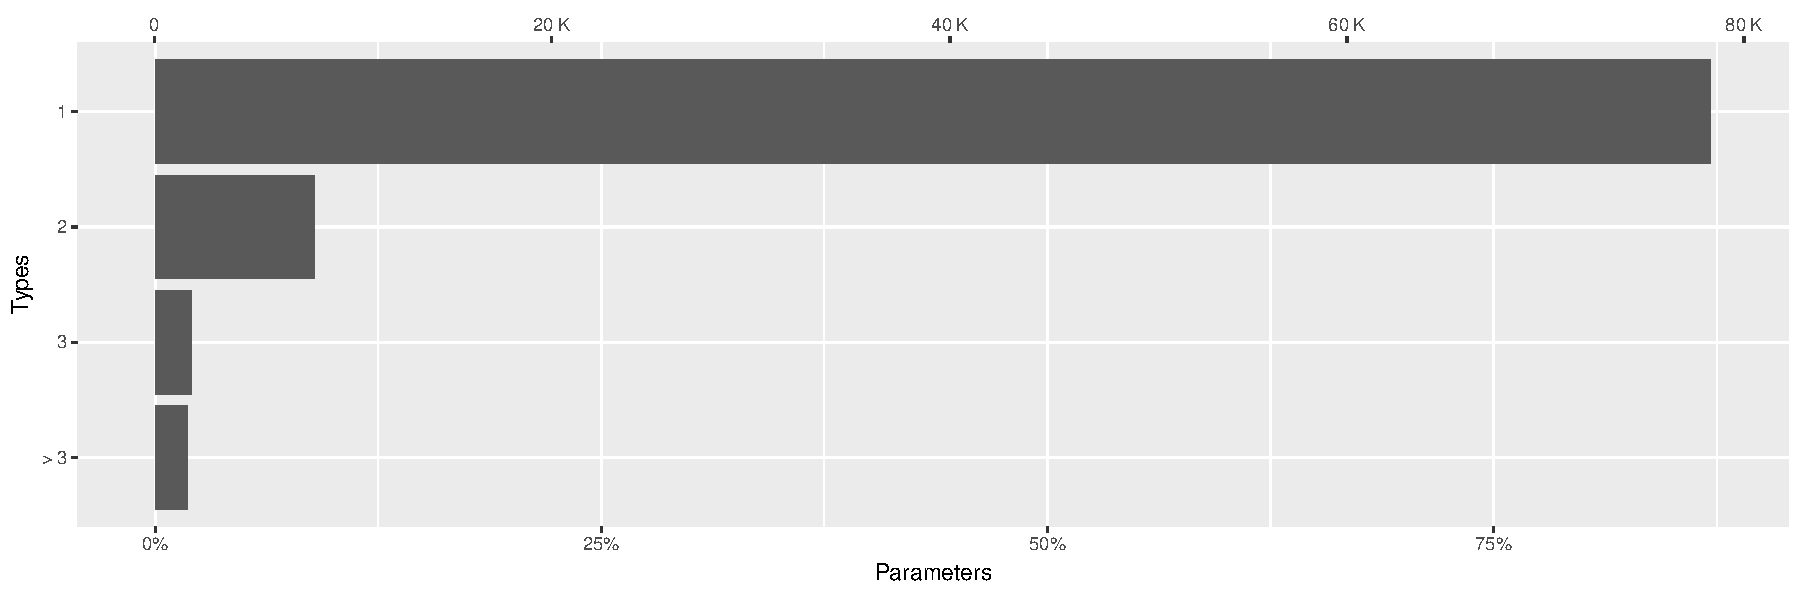
\includegraphics[width=.7\linewidth]{plots/union_frequency.pdf}
  \caption{Size of unions}\label{fig:unionfreq}
\end{figure}

First we look at the share of monomorphic arguments and function signatures.
Monomorphic in this context means that the type is not relying on \any or
including a union.  The import of monorphism in this context is that it
means our type language can accurately capture an argument's type or a
function signature. We get to that number in two steps.
Fig.~\ref{fig:unionfreq} shows the number of inferred argument types and
their size (in terms of terms in the union). The figure shows the most
functions do not require a union at all (\PercUnitypedPositions of arguments
do not have a union), and only \PercManytypedPositions positions have unions
with more than three members.


\begin{table}[H]
  \centering
  \resizebox{.5\linewidth}{!}{
    \begin{tabular}{lrrr}
      \toprule
      Types & Parameter \# & \% & Cumulative \%\\
      \midrule
      scalar & 35064 & 33.33 & 33.33 \\
      class & 24256 & 23.06 & 56.39 \\
      vector & 13025 & 12.38 & 68.77 \\
      \rowcolor{lightgray}  \textcolor{black}{...} & \textcolor{black}{9142} & \textcolor{black}{8.69} & \textcolor{black}{77.46}\\
      \rowcolor{lightgray} \textcolor{black}{null} & \textcolor{black}{7694} & \textcolor{black}{7.31} & \textcolor{black}{84.77}\\
        \addlinespace
   \rowcolor{lightgray}  \textcolor{black}{any} & \textcolor{black}{7614} & \textcolor{black}{7.24} & \textcolor{black}{92.01}\\
      \rowcolor{lightgray}  \textcolor{black}{list} & \textcolor{black}{3558} & \textcolor{black}{3.38} & \textcolor{black}{95.39}\\
      \textasciicircum{}vector & 2923 & 2.78 & 98.17\\
      function & 1427 & 1.36 & 99.52 \\
      environment & 500 & 0.48 & 100.00\\
      \bottomrule
    \end{tabular}}
  \caption{Singleton Type Categories}\label{fig:singlefreq}
\end{table}

The next step, is shown in Table~\ref{fig:singlefreq}, the table provides a
breakdown of types occuring in arguments without a union. Scalar, class and
vector are the most common type categories. The shaded rows correspond to
polymorphic types. Removing those gives us \CountMonomorphicPositions
(\PercMonomorphicPositions) monomorphic positions in a corpus of
\CountPositions parameters. With close to 70\% of monomorphic argument or
return values, it is fair to say that even a simple type language provides
significant benefits.

\begin{figure}[!h]  \centering
  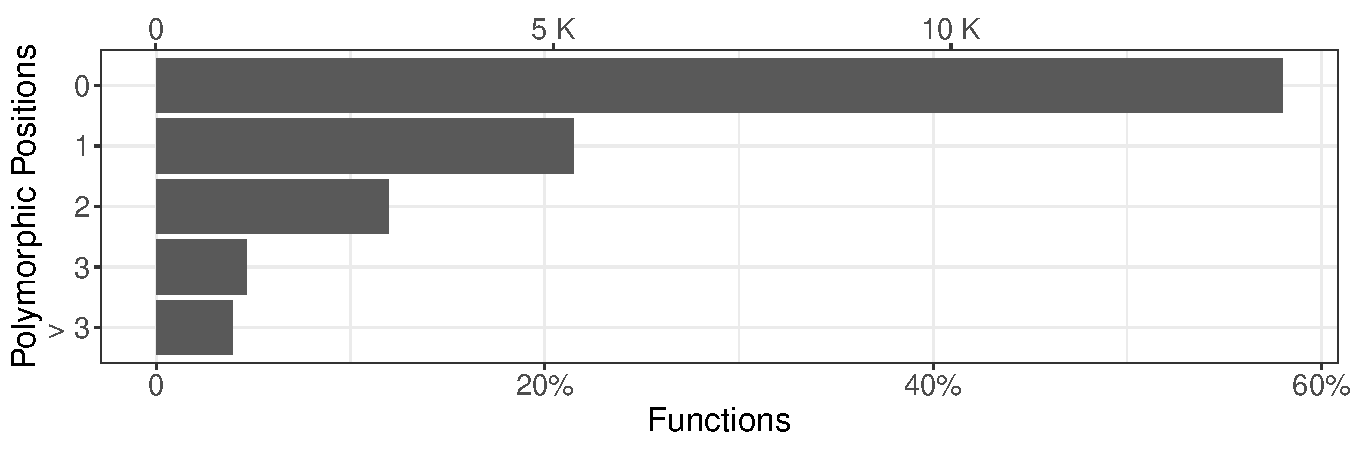
\includegraphics[width=.7\linewidth]{plots/function_polymorphism.pdf}
  \caption{Function Polymorphism}\label{fig:funpoly}
\end{figure}

If we look at the numbers from the point of view of functions and count how
many of their arguments are polymorphic, we observe that
\PercMonomorphicFunctions (\CountMonomorphicFunctions) functions are
monomorphic. The remaining \PercPolymorphicFunctions
(\CountPolymorphicFunctions) have at least one polymorphic parameter or
return type.  Figure~\ref{fig:funpoly} shows the distribution of functions
against the number of polymorphic arguments. Finally, we count
\CountMonomorphicPackages out of the 412 packages export only monomorphic
functions.

\subsubsection{Discussion}
A number of lessons can be drawn from the data we have gathered.

\paragraph{NAs}
Our data supports making the presence of {\NA}s explicit. Only 1,058 (of
0.9\%) of arguments are marked as possibly having {\NA}s, thus the
overwhelming majority of types appear to be {\NA}-free.  In practice,
programmers check for them and sanitize them if they are present.  Consider
the \code{binom} package for computing confidence intervals and its
\code{binom.profile} function.  This attached code snippet highlights a data
sanitization pattern: the programmer first binds the vectors into a matrix,
then finds rows where both columns are not \NA, extracts non-\NA values and
stores them into \code{x} and \code{n} respectively.

\begin{lstlisting}[basicstyle=\footnotesize\ttfamily]
  binom.profile <- function(x, n, conf.level=0.9, maxsteps=50,...) {
    xn <- cbind(x = x, n = n)
    ok <- !is.na(xn[, 1]) & !is.na(xn[, 2])
    x <- xn[ok, "x"]
    n <- xn[ok, "n"]
\end{lstlisting}

\paragraph{Scalars}
The data also suggests that programmers often use scalars, and do
dimensionality checks on their data.  In our data 31,533 (or 29\%) of the
arguments are scalar types. While not completely surprising, this is a
rather large number. Consider the \code{hankel.matrix} function, it takes
two arguments and checks that \code{n} is \int, that \code{x} is a vector,
and also, indirectly, that \code{n} is a a scalar (this comes from the fact
that it is used in the guard of a conditional which fails if \code{n} is
not a scalar).

\begin{lstlisting}[basicstyle=\footnotesize\ttfamily]
 hankel.matrix <- function( n, x ) { 
  ### n = a positive integer value for the order of the Hankel matrix
  ### x = an order 2 * n + 1 vector of numeric values
    if ( n != trunc( n ) )  stop( "argument n ix not an integer" )
    if ( !is.vector( x ) )  stop( "argument x is not a vector" )
    m <- length( x )
    if ( m < n )  stop( "length of argument x is less than n" )
\end{lstlisting}

\paragraph{Nullables}
The number of argument which may be \c{NULL} is 3,165 (or 3.5\%). This is a
relatively small number of occurrences, but it is worth expressing the
potential for the presence of \c{NULL} as these would likely inhibit
optimizations.

\paragraph{Structs}
While experimenting with various design, we consider adding a struct type to
capture lists with named elements that can be accessed with the \code{$}
operators. We ended discarding those types as they grew large and were often
only representative of the example data being manipulated.  Consider
function \code{cv.model}, its argument \code{x} is observed to be of
\CLASS{\texttt{aov}, \texttt{lm}} or \CLASS{\texttt{lm}}).  Internally,
linear models are represented as lists with named elements.  The polution is
illustrated by the lines after the funtion definition.  They load an example
data set and test the function \code{cv.model}.  The
\code{data(sweetpotato)} expression load a sample data set. The fields of
\code{sweetpotato} will be recorded when \code{cv.model} is called.

\begin{lstlisting}[basicstyle=\footnotesize\ttfamily]
  cv.model <- function(x) {
    suma2 <- sum(x$residual^2)
    gl <- x$df.residual
    promedio <- mean(x$fitted.values)
    return(sqrt(suma2/gl)*100/promedio)
  }
  
  data(sweetpotato)
  model<-aov(yield~virus, data=sweetpotato)
  cv.model(model)
\end{lstlisting}


\paragraph{Objects}
While we record classes, our analysis does not deal with method dispatch.  R
has multiple, disparate, object systems, called S3, S4, and R5.  The
\code{class} attribute is used by these systems to dispatch methods. S3 does
single dispatch, S4 does multiple dispatch and R5 supports impertative
objects.  The mechanics of S4 dispatch are more complex than for S3, and
users can define their own class hierarchies that we would need to
incorporate in our type analysis and contract checking frameworks.  We found
limited use of S4 during our analysis. Coming up with a type system that
accounts for all of these factors and consolidates multiple
object-orientation frameworks in a single language design is an interesting
problem in and of itself, one we leave for future work.  

\paragraph{Matrices}
Matrices are instances of the eponymous class. They have a \code{dims}
attribute indicating dimensions, and while not codified in the language
semantics, many internal functions coerce vectors to matrices automatically.
The \code{rowWeightedMeans} function calculates the weighted means of rows.
The programmer added a type check for \code{x}.

\begin{lstlisting}[basicstyle=\footnotesize\ttfamily]
  rowWeightedMeans <- function(x, w=NULL, rows=NULL, cols=NULL, na.rm=FALSE, ...) {
    if (!is.matrix(x))   .Defunct(msg = sprintf("'x' should be a matrix.)
\end{lstlisting}


\paragraph{Data Frames}
One of the most popular classes in R is the \code{data.frame} class, making
up nearly 8\% of observed classes.  Data frames and the derivative
\code{tibble} and \code{data.table} types underpin many popular uses of R.
One way to deal with data frames is through the struct type, with a named
field for each column of the data frame, but as mentioned previously structs
introduced undue noise.  Further complicating data frames is that many
functions built to operate on them operate in a name-agnostic way.  For
instance, the \code{tidyverse} package ecosystem allows programmers to pass
column names to functions which operate on their data frames.  In base R,
idiomatic data frame use is to use string column names to select rows from
the frame (unless only a single column is of interest, wherein the \code{$}
syntax is appropriate).

\subsection{Robustness}

How robust are the inferred types?  To measure this, we conducted another
large-scale experiment: for each package in the corpus, we ran used the
inferred type signatures as contracts and ran all of the CRAN reverse
dependencies for that package. In total we ran \NUMPKGSEVAL packages and
recorded \NUMASSERTIONS total assertions.  Overall, we found that only
\PERCFAILEDASSERTIONSWUNDEF of contract failed.  The limit on number of
arguments (we record only 20) accounted for \PERCASSERTIONSUNDEF failed
assertion. We found that \PERCSUCCARG of parameter types and \PERCSUCCFUNS
of functions types never failed.  The number of immaculate function types
increases to \PERCSUCCFUNNOSTHREE if we discount S3 object method dispatch.
Overall, these numbers are promising, and suggest that the type signatures
are robust.

We breakdown the failed assertions by type in
Table~\ref{tbl:fail-breakdown-0}.  Accounting for 27\% of assertion
failures, is when \CLASS{\texttt{matrix}} is passed where a \VEC\dbl is
expected.  Considering these types, we might imagine them to be compatible,
however not allowing this coercion was a deliberate design decision:
coercion from vectors to matrices is ad hoc at best, and surely not a
practice codified in the language.  In a similar vein, another popular
failing assertion is checking if a ${\bf dbl}[]$ has type ${\bf int}[]$,
another case of commonly performed coercion.  We did not include these types
of coercions in our type annotation framework as programmers cannot rely on
them, and it is not always the case that the coercions are safe to perform.

\begin{table}
% BEGIN Autogenerated
\small
\begin{tabular}{llrrr}
\toprule
Passed & Arg Type & Occurrences & \% Total & Cumulative \%\\
\midrule
\VEC\dbl & \CLASS{\texttt{matrix}} & 371,896 & 27.37 & 27.37\\
\VEC\dbl & \VEC\int & 117,212 & 8.62 & 35.99\\
\chr & \CLASS{\texttt{bignum}} | \VEC\raw & 100,100 & 7.37 & 43.36\\
\dbl & \int | \null & 60,578 & 4.46 & 47.81\\
\VEC\dbl & \CLASS{\texttt{timeSeries}} & 58,872 & 4.33 & 52.15\\
\addlinespace
\CLASS{\texttt{matrix}} & \CLASS{\texttt{timeSeries}} & 55,005 & 4.05 & 56.19\\
\VEC\dbl & \dbl & 53,338 & 3.92 & 60.12\\
\dbl & \CLASS{\texttt{data.frame}} & 32,553 & 2.40 & 62.51\\
\VEC\dbl & \CLASS{\texttt{data.frame}} & 31,576 & 2.32 & 64.84\\
\dbl & \int & 20,586 & 1.51 & 66.35\\
\bottomrule
\end{tabular}
% END Autogenerated
\label{tbl:fail-breakdown-0}\caption{Top contract failures}\end{table}

In addition to the number of failed contract checks, we were interested in
how many functions had a parameter where a contract check failed, and
overall we found this to be the case in \PROPFUNSFAILEDCHECK of functions.
Digging a little deeper, we noticed that many of these functions were
performing S3 dispatch which we do not handle.  Removing those functions, we
see that \PROPFUNSFAILEDCHECKNOSTHREE of functions exhibited failing
contract checks.  These are functions were likely under-tested, as calls to
these functions represent only \PERCCALLSBADFUNSINTESTS of recorded calls
during \typetracer's run on the core corpus to infer types.

Turning our attention now to arguments, we found that only
\PROPARGSFAILINGASSERTS of parameters failed.
Table~\ref{tbl:fail-breakdown-0} showed the runtime occurrences, but that
data alone does not tell the full story, as some failures may be
overrepresented if e.g. a failing contract assertion was in a loop.  We were
interested in knowing for each of the most common violations in
Table~\ref{tbl:fail-breakdown-0}, how many different arguments had that
type, and how many of those exhibited the contract failure in question.
Table~\ref{tbl:fail-breakdown-1} breaks down the failed assertions by type,
folding away multiple identical failed contract assertions for the same
parameter position.  The first row of this table reads: a value of type
\VEC\dbl was passed to 15 different function parameters expecting a
\CLASS{\texttt{matrix}}, of which there are 1394 in total: 1\% of
\CLASS{\texttt{matrix}}-typed parameters were passed \VEC\dbl values.

We see that even though the double vector and matrix issue was wildly
prevalent in the raw, dynamic contract evaluation numbers, the number of
actual function argument types that were violated is very small.  The story
is similar with the double and integer coercion we mentioned earlier: it
represents many dynamic contract failures, but very few of the
\VEC\int-typed arguments have their contracts violated by \VEC\dbl-typed
values.  Rows 5 and 6 are interesting: we see that rather often arguments
expecting \CLASS{\texttt{timeSeries}} data are passed \VEC\dbl or
\CLASS{\texttt{matrix}} values.  This is a quirk of the \code{timeSeries}
package, whose functions often accept matrices and vectors, converting them
to time series in an ad hoc manner.  Note that the code coverage of the
\code{timeSeries} tests, examples, and vignettes on the \code{timeSeries}
package code is only 58\%, which is one possible explanation of why these
contract failures are occurring: the types that \typetracer generates are
only as good as the test code its run on.

 \begin{table}
% BEGIN Autogenerated
\small
\begin{tabular}{llrrr}
\toprule
Passed & Arg Type & \# Args Failed & \# Args with Type & \% Failure\\
\midrule
\VEC\dbl & \CLASS{\texttt{matrix}} & 15 & 1394 & 1.08\\
\VEC\dbl & \VEC\int & 44 & 657 & 6.70\\
\chr & \CLASS{\texttt{bignum}} | \VEC\raw & 1 & 3 & 33.33\\
\dbl & \int | \null & 5 & 20 & 25.00\\
\VEC\dbl & \CLASS{\texttt{timeSeries}} &19 & 35 & 54.29\\
\addlinespace
\CLASS{\texttt{matrix}} & \CLASS{\texttt{timeSeries}} &  19 & 35 & 54.29\\
\VEC\dbl & \dbl & 100 & 5021 & 1.99\\
\dbl & \CLASS{\texttt{data.frame}} &  1 & 900 & 0.11\\
\VEC\dbl & \CLASS{\texttt{data.frame}} &  6 & 900 & 0.67\\
\dbl & \int & 48 & 529 & 9.07\\
\bottomrule
\end{tabular}

% END Autogenerated
 \label{tbl:fail-breakdown-1}
 \caption{Results from Table~\ref{tbl:fail-breakdown-0}, broken down by occurrences of the expected type as a parameter type}
 \end{table}

Table~\ref{tbl:fail-breakdown-2} presents data on the most frequently
violated contracts amongst the most frequently occurring argument types.  We
selected argument types which were in the 90th percentile of argument type
occurrences, computed the most frequent type signature violations among
them, and reported the most frequently violated contracts together with the
type of the value that violated that contract.  The first row of the table
reads: 44 function arguments with \VEC\int type are passed \VEC\dbl instead,
and 657 arguments have \VEC\int type.  Had we failed to capture some key
usage pattern of R with our type annotation framework, we would likely see
it here, and we can see this in action if we consider
Table~\ref{tbl:fail-breakdown-3}, which was obtained identically to
Table~\ref{tbl:fail-breakdown-2} with a percentile of 80th percentile
instead.  The most frequent argument type violation pattern in that of
\CLASS{\texttt{data.frame}} values passed to arguments expecting tibbles,
which are an extension of \CLASS{\texttt{data.frame}} built in the
\code{tidyverse} package suite: this occurs in only 22\% of such arguments,
and represents cases where tests did not adequately cover all valid function
inputs.  Separate from the issue of testing, we can capture this behaviour
with user-defined subtyping, as data frames are subtypes of tibbles, but
this necessitates a proper object-oriented type system for R which is
outside the scope of this work.

 \begin{table}
% BEGIN Autogenerated\
\small
\begin{tabular}{llrrr}
\toprule
Passed & Arg Type & \# Args Failed & \# Args with Type & \% Failure\\
\midrule
\VEC\dbl & \VEC\int & 44 & 657 & 6.70\\
\NAVEC\lgl & \null & 158 & 2756 & 5.73\\
\VEC\chr & \chr & 183 & 4102 & 4.46\\
\chr & \null & 117 & 2756 & 4.25\\
\dbl & \null & 107 & 2756 & 3.88\\
\bottomrule
\end{tabular}
% END Autogenerated
 \label{tbl:fail-breakdown-2}
 \caption{What is the highest failure rate among popular argument types? For argument signatures whose frequency is in the 90th percentile}
 \end{table}
 
  \begin{table}
% BEGIN Autogenerated
\small
\begin{tabular}{ll@{}rrr@{}}
\toprule
Passed & Arg Type & \#Args Fail & \#Args w Type & \% Failure\\
\midrule
\CLASS{\texttt{data.frame}} & \CLASS{\texttt{data.frame}, \texttt{tbl}, \texttt{tbl\_df}} & 63 & 284 & 22.18\\
\CLASS{\texttt{matrix}} & \CLASS{\texttt{array}} & 13 & 70 & 18.57\\
\NAVEC\lgl & \lgl | \null & 9 & 49 & 18.37\\
\VEC\chr & \LIST{\VEC\chr} & 20 & 109 & 18.35\\
\VEC\clx & \clx & 7 & 42 & 16.67\\
\bottomrule
\end{tabular}
% END Autogenerated
 \label{tbl:fail-breakdown-3}
 \caption{What is the highest failure rate among popular argument types? For argument signatures whose frequency is in the 80th percentile}
 \end{table}
 
In sum, we believe that this evaluation shows that the type signatures we
generate from traces are quite good.  Only \PERCFAILEDASSERTIONSWUNDEF of
contract assertions failed at runtime, representing failures in as few as
\PROPARGSFAILINGASSERTS of argument types.  Even though
\PROPFUNSFAILEDCHECKNOSTHREE of functions had at least one argument type
involved in a failing contract check, these functions are under-tested,
representing only \PERCCALLSBADFUNSINTESTS of calls observed while inferring
types.
 
%
%
%
%
\subsection{Usefulness of the Type Checking Framework}

There is a number of ways in R to check types of function parameters. The
default and the most common way\footnote{\CranStopifnotRatio of all runtime
  checks in the whole of CRAN} is to use \code{stopifnot} function from the R
base package. It takes a number of R expressions which all should evaluate to
true otherwise a runtime exception is thrown with a message quoting the
corresponding failed expression. For example, the following code checks whether
a given parameter \code{x} is a scalar string:
%
\begin{lstlisting}
stopifnot(is.character(x), length(x) == 1L, !is.na(x))
\end{lstlisting}

Next to \code{stopifnot}, there are 4 packages in CRAN\footnote{Packages are
  available on CRAN website: \url{https://cran.r-project.org/web/packages/}}.
that focus on runtime assertions: \emph{assertive}, \emph{ensurer},
\emph{assertr} and \emph{assertthat} \emph{assertive} and \emph{ensurer} have
not been updated 2016 and 2015 respectively. \emph{assertr} is used by only
\AssertrRevdeps other packages and in the current version focuses on checking
properties of data frames. Only the \emph{assertthat} is maintained and used
(with \AssertthatRevdeps reverse dependencies). The advantage of
\emph{assertthat} over the R's default is that it provides a much better error
message.

One way to asses the usefulness of our type checking system is to find out how
many of the existing type checking constrains could be replaced by \contractr.
To measure this, we have extracted all calls to \code{stopifnot} and
\code{assertthat} assertions and checked which one of them could be either
completely replaced by \contractr or at least partially simplified by removing a
portion of an assertion expression. This is useful, because a common pattern is
that the first part of the parameter assertion checks its type while the rest
checks its value. In the example above, the whole expression could be replaced
by \code{character} type.

Out of the \CorpusLoadable packages, \CorpusAssertsInPackages use runtime
assertions. Together there are \CorpusAsserts asserts in
\CorpusAssertsInFunctions functions. Among these, \contractr can replace
\CorpusTypedAsserts (\CorpusTypedAssertsRatio) assertion calls across
\CorpusTypedAssertsPackages packages and \CorpusTypedAssertsFunctions functions.
Furthermore, additional \CorpusPartiallyTypedAsserts
(\CorpusPartiallyTypedAssertsRatio) asserts in packages
\CorpusPartiallyTypedAssertsPackages packages and
\CorpusPartiallyTypedAssertsFunctions functions could have been simplified.

Checking the type of function parameters is not something that is seen often in
the R code. In the whole of CRAN, there are only \CranAssertsRnd asserts in
\CranAssertsInFunctionsRnd functions define in \CranAssertsInPackagesRnd
packages. One might speculate that one of the reasons is that the current way is
not convenient as it is rather verbose. Our system can infer type annotations
for existing functions automatically. This can remove or partially remove over
\CorpusPartiallyTypedAssertsRatio of existing assertions.

\section{Conclusion}

Our goal with this work was to ...

Overall, we found that our proposed design fits quite well with the existing language:
Over 82\% of functions are either monomorphic or have only one single polymorphic argument, indicating that our design fits quite well with the language.
When we tested the types inferred by \typetracer during our evaluation, we found that only \PERCFAILEDASSERTIONSWUNDEF of contract assertions failed, and found no pathological patterns in argument types with failed assertions.
Furthermore, we found that our type language and contract checking framework could eliminate or otherwise simplify \CorpusPartiallyTypedAssertsRatio of existing type checks and assertions in user code.

\bibliography{bib/biblio,bib/jv,bib/r,bib/new,bib/gradual}
\end{document}
